\section{Dataset Statistics}
\label{app:data}

We briefly summarize the main dataset statistics used in our experiments; full counts and scripts are provided in the anonymized supplementary repository.

\paragraph{Weibo.} We use the standard multimodal Weibo rumor dataset with paired images and Chinese text. Following prior work, we adopt the official event-disjoint split into train/dev/test and keep the natural class imbalance (real vs.~fake). Event IDs correspond to curated rumor stories; the number of events and posts per split, as well as the proportion of small events (fewer than five posts), are reported by our data-preprocessing script.

\paragraph{WeChat / WeFEND.} The WeFEND corpus contains 7,231/905/905 public-account articles in the train/dev/test splits, each with a cover image and metadata. Events are defined by public-account story IDs or linked fact-check articles. We follow the chronological split from the original release to avoid leakage; per-split class imbalance and image coverage are summarized in our released statistics.

\section{Additional Results and Analysis}
\label{app:results}

\paragraph{Text-only and image-only baselines.} In addition to the multimodal baselines reported in Table~\ref{tab:main}, we include text-only BERT and image-only ViT models. On Weibo, text-only BERT is competitive with multimodal SAFE/EANN, while image-only ViT is substantially weaker; on WeFEND, text-only BERT lags behind multimodal baselines in both Macro--F1 and ECE. These trends support our focus on multimodal fusion and reliability-aware distillation.

\paragraph{Fakeddit experiments.} We conducted preliminary experiments on the English Fakeddit benchmark under a strict time-split protocol that prevents events from leaking across train and test. In this challenging setting, all content baselines achieve relatively low accuracy: text-only BERT reaches Acc/Macro--F1 of about 0.54/0.54 (ECE~0.33), image-only models perform worse (0.46/0.46, ECE~0.40), EANN attains roughly 0.51 Macro--F1 (ECE~0.38), and a RoBERTa-large + ViT-large fusion teacher averages about 0.50/0.50 with ECE~0.38 across seeds. A student trained with \modelname{} closely tracks the teacher (Macro--F1 $\approx$ 0.50, ECE $\approx$ 0.39), and a SpotFake+-style model (BERT-base + ResNet101 with cross-modal attention) performs even worse (Acc/Macro--F1 $\approx$ 0.49/0.49, ECE~0.42). These findings confirm that our strict Fakeddit configuration is substantially harder than commonly used random splits and that, with such weak teachers, DMPD cannot deliver consistent accuracy gains. We therefore treat strict Fakeddit as a hard case and leave a more thorough study, including graph-based and VLM-based detectors, to future work; our main paper focuses on settings where teachers are competitive but imperfect (Weibo, WeFEND, MiRAGeNews).

\paragraph{MiRAGeNews stress test.} To probe cross-generator robustness on English synthetic news, we also evaluate \modelname{} on MiRAGeNews, which contains real and AI-generated news-style posts with paired images. The teacher achieves near-saturated performance on the in-distribution split (Acc/Macro--F1 $\approx 0.996$) but degrades on cross-generator test subsets where the text or image generator changes. Averaged over the four out-of-distribution subsets and three seeds, the student improves accuracy and Macro--F1 from roughly 0.88 to 0.90 (about +2 points) and slightly reduces ECE (from $\approx 0.057$ to $\approx 0.053$). Because MiRAGeNews lacks explicit event IDs, we only use instance-level gating there; the results suggest that our gated distillation remains beneficial under distribution shift, while full calibration for synthetic generators is an interesting direction for future work.

\paragraph{MiRAGeNews temperature variants (not used in main table).} We tried two temperature tweaks. (i) Higher-$T$ (initial $T{=}2.5$ with stronger augmentation): averaged over two seeds, OOD test2--5 yields Acc 0.918 / Macro--F1 0.918 with ECE 0.0585—slightly higher accuracy but worse calibration than the main 3-seed setting (ECE $\approx 0.053$). (ii) Lower-$T$ (initial $T{=}2.0$): three seeds (05/06/07) give OOD Acc 0.9020 / Macro--F1 0.9017 / ECE 0.0506 (std $\approx$ 0.013/0.013/0.0012); per-split ECE varies (e.g., test3 ECE 0.091). We keep the main multi-seed configuration in Table~\ref{tab:main} and report these temperature variants as calibration trade-offs.

\paragraph{Synthetic label noise (Weibo).} We inject controlled label/event noise (rates 0.1/0.2/0.3) on Weibo to test robustness. With heavy noise (0.2--0.3), \modelname{} and full-KD Noisy-Student yield nearly identical Macro--F1 and ECE; with lighter noise (0.1), \modelname{} attains slightly lower ECE at comparable accuracy. Detailed numbers are in \texttt{paper\_results/weibo\_noise\_comparison.csv} and serve as a sanity check rather than a main claim.

\paragraph{Simple confidence-gated KD.} As a stronger KD baseline, we implement a simple confidence-based scheme in which the student distills from the fusion teacher whenever its confidence exceeds a fixed threshold, without cross-view agreement or event-level reliability. On Weibo, simple confidence-gated KD achieves Macro--F1 $\approx 0.942$ and ECE $\approx 0.043$ (mean over three seeds), compared to $\approx 0.948$ and ECE $\approx 0.040$ for \modelname{}. On WeFEND, simple confidence-gated KD attains Macro--F1 $\approx 0.905$ and ECE $\approx 0.053$, while \modelname{} reaches $\approx 0.913$ with ECE $\approx 0.030$. These results confirm that combining cross-modal agreement with event-aware filtering is more effective than per-instance confidence thresholds alone.

\paragraph{Illustrative error cases (Weibo test).} Without revealing text/images, we list two representative outcomes comparing the fusion teacher and the \modelname{} student:
\begin{itemize}
  \item \textbf{Teacher confidently wrong, student correct:} label = fake; teacher predicts \emph{real} with confidence 0.988; student predicts \emph{fake} with confidence 0.995.
  \item \textbf{Teacher correct, student over-confidently wrong:} label = real; teacher predicts \emph{real} with confidence 0.758; student predicts \emph{fake} with confidence 0.996.
\end{itemize}
These cases illustrate both the benefit (filtering confident teacher errors) and the remaining risk (student over-confidence when a wrong signal is admitted), motivating agreement-aware gating and calibration.

\paragraph{Teacher--student error quadrants.} We further break test samples into four quadrants by teacher/student correctness and report proportions and mean cross-modal disagreement $|p_\text{text}-p_\text{image}|$ (CSV: \texttt{paper\_results/error\_quadrant\_stats.csv}). On Weibo: T-wrong/S-right 1.39\%, T-right/S-wrong 0.96\%, T-wrong/S-wrong 3.31\%, T-right/S-right 94.34\%. On WeFEND the pattern is similar (2.32/1.44/4.20/92.04\%). High disagreement concentrates in the error quadrants, supporting the use of agreement-aware selective distillation. Per-sample event reliability was not available in the stored predictions, so we omit that statistic.

\paragraph{Per-class calibration (Weibo/WeFEND).} For the main student and fusion teacher, we report per-class ECE (15 bins) and NLL:
\begin{itemize}
  \item Weibo: student per-class ECE $(\text{real},\text{fake}) = (0.036, 0.036)$; teacher $(0.040, 0.040)$; NLL (student/teacher) = 0.227 / 0.189.
  \item WeFEND: student per-class ECE $(0.042, 0.042)$; teacher $(0.046, 0.046)$; NLL (student/teacher) = 0.230 / 0.222.
\end{itemize}
These numbers indicate that \modelname{} does not degrade calibration relative to the fusion teacher and slightly improves per-class ECE on WeFEND, while Weibo NLL remains competitive despite the student being sharper.

\paragraph{Cross-modal disagreement vs.~error.} We quantify disagreement as $|p_{\text{text}}(\text{fake}) - p_{\text{image}}(\text{fake})|$ and bin samples into deciles; the error rate is computed from the student predictions. Figure~\ref{fig:disagree} shows that higher disagreement correlates with higher error on both Weibo and WeFEND, motivating the use of agreement-aware gating. Underlying bucketed statistics are released alongside the plots.

\begin{figure}[t]
  \centering
  \IfFileExists{figures/disagreement_error.pdf}{%
    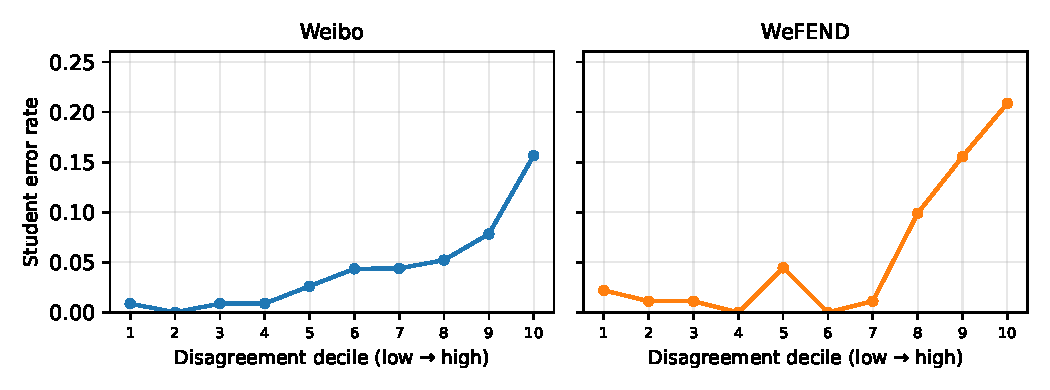
\includegraphics[width=0.95\linewidth]{figures/disagreement_error.pdf}%
  }{%
    \fbox{\rule{0pt}{120pt}\rule{0.95\linewidth}{0pt}}%
  }
  \caption{Student error rate vs.\ cross-modal disagreement deciles on Weibo and WeFEND (decile 1 = lowest disagreement).}
  \label{fig:disagree}
\end{figure}

\paragraph{Loose gate coverage.} To verify that gating can open on Weibo when thresholds are relaxed, we run a loose configuration (e.g., $\tau_f{=}0.90$, $\tau_m{=}0.85$, $\delta{=}0.10$, warmup $=0$, small margin). Figure~\ref{fig:loosegate} plots the number of distill pairs per epoch: coverage becomes non-zero on both Weibo and WeFEND, while test performance remains close to the main configuration (Weibo Acc/Macro--F1/ECE $\approx$ 0.947/0.947/0.046; WeFEND 0.935/0.904/0.056). This confirms that the gating logic is functional even when relaxed.

\begin{figure}[t]
  \centering
  \IfFileExists{figures/gate_coverage_loose.pdf}{%
    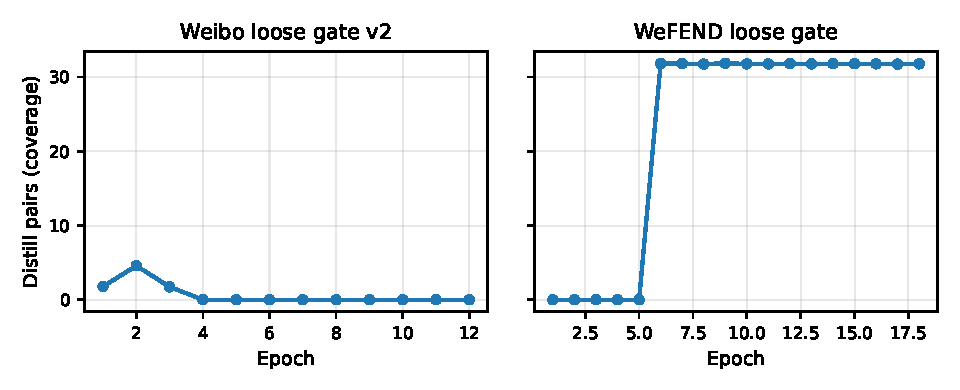
\includegraphics[width=0.95\linewidth]{figures/gate_coverage_loose.pdf}%
  }{%
    \fbox{\rule{0pt}{120pt}\rule{0.95\linewidth}{0pt}}%
  }
  \caption{Distill coverage (num\_distill\_pairs) over epochs with looser thresholds on Weibo and WeFEND.}
  \label{fig:loosegate}
\end{figure}

\paragraph{Coverage--performance trade-off.} Using the same sweep points as Table~\ref{tab:main} variants (WeFEND gate A/B/C and the main setup, plus Weibo main and loosegate v2), Figure~\ref{fig:coverage-perf} plots coverage vs.\ Macro--F1 and coverage vs.\ ECE (data in \texttt{paper\_results/coverage\_perf\_points.csv}). On WeFEND, higher coverage (point B) yields slightly higher Macro--F1 but worse ECE; lower-coverage points (A/C) improve calibration at a small F1 cost. On Weibo, loose gating increases coverage modestly (mean $\approx 0.68$) but slightly raises ECE.

\begin{figure}[t]
  \centering
  \IfFileExists{figures/coverage_vs_mf1.png}{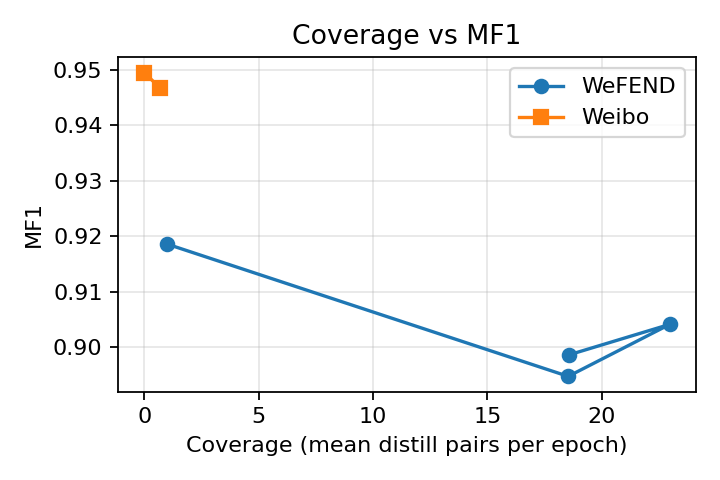
\includegraphics[width=0.47\linewidth]{figures/coverage_vs_mf1.png}}{\fbox{\rule{0pt}{90pt}\rule{0.47\linewidth}{0pt}}}
  \hfill
  \IfFileExists{figures/coverage_vs_ece.png}{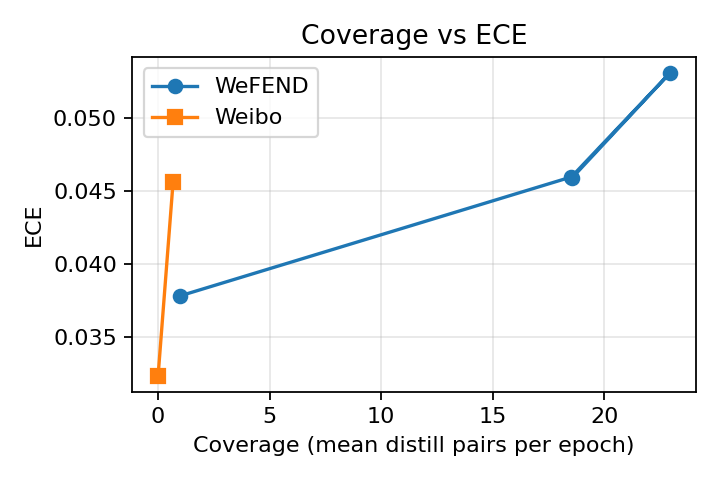
\includegraphics[width=0.47\linewidth]{figures/coverage_vs_ece.png}}{\fbox{\rule{0pt}{90pt}\rule{0.47\linewidth}{0pt}}}
  \caption{Coverage vs.\ Macro--F1 (left) and Coverage vs.\ ECE (right) for WeFEND gate sweep (A/B/C/main) and Weibo (main, loosegate v2). Higher coverage can raise Macro--F1 but may worsen calibration; lower coverage tends to reduce ECE.}
  \label{fig:coverage-perf}
\end{figure}

\paragraph{WeFEND gate sweep (coverage--performance trade-off).} We sweep gate thresholds on WeFEND to inspect the coverage/accuracy trade-off. Point A $(\tau_f{=}0.93,\ \tau_m{=}0.88,\ \delta{=}0.07)$ attains Acc 0.928 / Macro--F1 0.895 / ECE 0.046 with mean coverage 18.53 distill pairs per epoch. Point B $(0.90,\ 0.85,\ 0.10)$ yields Acc 0.935 / Macro--F1 0.904 / ECE 0.053 with higher mean coverage 22.97. The main configuration lies between these settings; A is better calibrated, B covers more samples.
\paragraph{WeFEND gate sweep (coverage--performance trade-off).} We sweep gate thresholds on WeFEND to inspect the coverage/accuracy trade-off. Point A $(\tau_f{=}0.93,\ \tau_m{=}0.88,\ \delta{=}0.07)$ attains Acc 0.928 / Macro--F1 0.895 / ECE 0.046 with mean coverage 18.53 distill pairs per epoch. Point B $(0.90,\ 0.85,\ 0.10)$ yields Acc 0.935 / Macro--F1 0.904 / ECE 0.053 with higher mean coverage 22.97. Point C $(0.92,\ 0.87,\ 0.08)$ gives Acc 0.933 / Macro--F1 0.899 / ECE 0.046 with mean coverage 18.54. The main configuration lies between these settings; A/C are better calibrated, B covers more samples.

\paragraph{WeFEND bar chart (from Table~\ref{tab:main}).} For a visual summary of WeFEND results, Figure~\ref{fig:wefend-bar} plots Macro--F1 and ECE for text-only, SAFE, EANN, the fusion teacher, and \modelname{}, using exactly the numbers reported in Table~\ref{tab:main}. The plot highlights that \modelname{} yields the highest Macro--F1 and the lowest ECE among these baselines.

\begin{figure}[t]
  \centering
  \IfFileExists{figures/wefend_bar.pdf}{%
    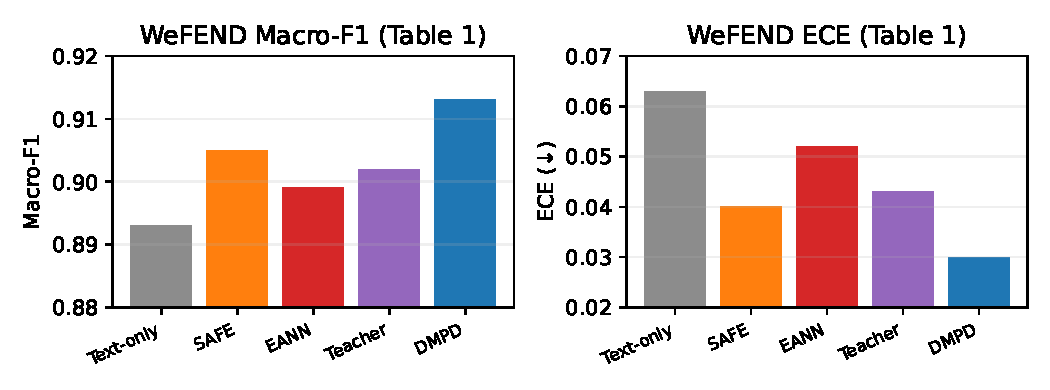
\includegraphics[width=0.95\linewidth]{figures/wefend_bar.pdf}%
  }{%
    \fbox{\rule{0pt}{120pt}\rule{0.95\linewidth}{0pt}}%
  }
  \caption{WeFEND Macro--F1 and ECE for key baselines and \modelname{}, derived directly from Table~\ref{tab:main}.}
  \label{fig:wefend-bar}
\end{figure}

\paragraph{Selector ablations.} We also ablate the modality selector that chooses which unimodal branch to pair with the fusion teacher. On Weibo and WeFEND, always selecting the text branch or always selecting the vision branch yields lower Macro--F1 and worse calibration than our confidence-based selector. For example, on WeFEND (one seed), the confidence-based selector attains Acc 0.930, Macro--F1 0.898, and ECE 0.033, compared to 0.919/0.881/0.042 for always-text and 0.928/0.895/0.061 for always-vision, supporting the use of dynamic modality priority.

\paragraph{Significance and robustness.} For Weibo, the improvements of \modelname{} over EANN are statistically significant under both paired bootstrap and McNemar's test (Section~\ref{sec:experiments}). For WeFEND, we report mean $\pm$ standard deviation over multiple seeds and observe consistent gains in Macro--F1 and ECE; per-seed curves and additional reliability diagrams are available in the anonymized repository.

\section{Implementation Details}
\label{app:impl}

We implement all models in PyTorch using BERT and ViT encoders with a lightweight fusion head. Training hyper-parameters (learning rates, weight decay, batch sizes, and schedules) are specified in the released YAML configurations. All experiments are run on a single modern GPU per run; wall-clock training times and exact seeds are logged and summarized by the scripts in the anonymized repository. Teachers are pretrained separately and kept frozen during distillation; only student parameters are updated. We also release small utilities to regenerate all tables and figures from saved JSON summaries and prediction files.
